  \chapter{Conditional Generation of Linkages}\label{ch-cave-linkage}
\section{Introduction}
 In this chapter we present an alternate End-to-End deep neural network architecture for Variational Synthesis of linkages. This End-to-End architecture is a Conditional-VAE (C-VAE), which approximates the conditional distribution of linkage parameters with respect to coupler trajectory distribution. The outcome is a probability distribution of kinematic linkages for an unknown coupler path or motion. This framework functions as a bridge between the current state of the art theoretical and computational kinematic methods and  machine learning to enable designers to create practical mechanism design solutions.
 
 This chapter presents a generative way of learning End-to-End synthesis for planar linkages using C-VAE. A case study of End-to-End Variational Synthesis using pure Deep Learning is presented in Section~\ref{cvae-case-study}.
 

\begin{figure}
\centering
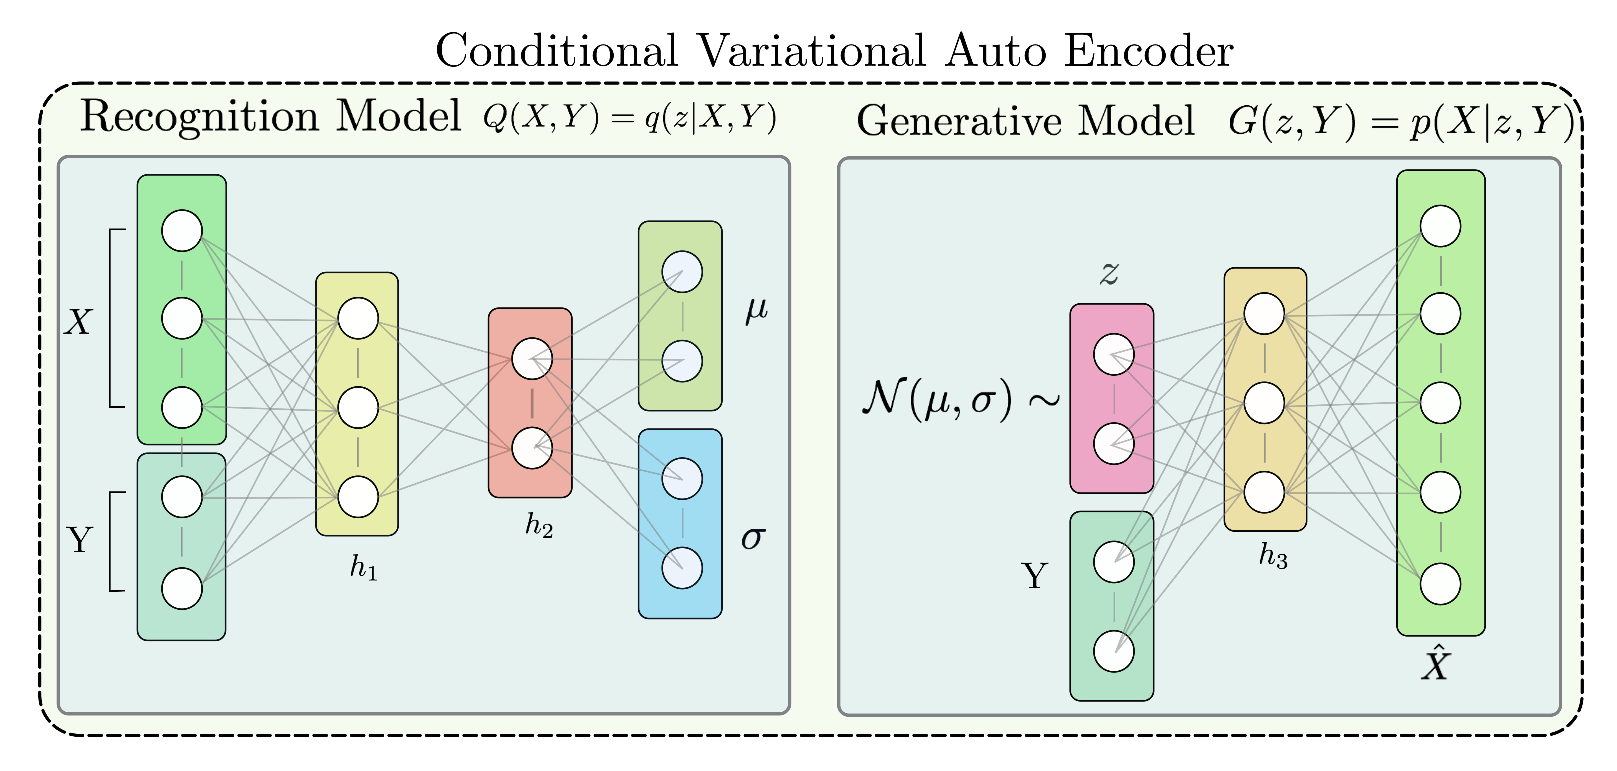
\includegraphics[width=250pt]{jmd-19/figure/fig_cvae.eps}
  \caption{Recognition Model encodes the observed data $X$ and observed property $Y$ into probabilistic latent coding $z$ of dimension much smaller than $X$. In this case, we assume a multivariate Gaussian distribution for $z$. Generative Model takes samples from this distribution and combines it with $Y$ to generate output $\hat{X}$}
\label{cvae_arch}
\end{figure}

 
\section{Conditional Variational Auto Encoders (C-VAE)}\label{sec_condi_vae}

C-Variational Auto Encoders (C-VAE)~\cite{Kingma2014AutoEncodingVB} is a neural network architecture that learns to approximate conditional distribution of an observed data $X$ given an observed property $Y$.
Figure~\ref{cvae_arch} shows a general architecture of a C-VAE.
In this figure, $X$ and $Y$ are concatenated and fed to Recognition Model as the input. There are two hidden layers $h_1$ and $h_2$ in the Recognition Model, while the Generative Model has one hidden layer $h_3$. In the middle, there is feature space encoded by the variable $z$, which seeks to capture the salient features of the input data in a compact latent space.
Given observed variables $X$ and $Y$, Recognition Model computes a approximate probability distribution $q(z|X, Y)$ of the latent variable $z$ as following:
\begin{eqnarray}\label{eq_Q_cvae}
\mu, \sigma = Q(X, Y; \theta_e),\\
  q(z|X) = \mathcal{N}(\mu, \sigma).\label{eq_Q_2}
\end{eqnarray}
Here, $\mathcal{N}(\mu, \sigma)$ is a multivariate Gaussian distribution function with mean $\mu$ and variance $\sigma$.
The generative model is a function which is trained to maximize likelihood samples $\hat{X}$ by taking a sample from $z \in q(z|X, Y)$ and concatenating it with $Y$. Thus, $X$ is given by,
\begin{equation}\label{eq_cvae}
  \hat{X} = G(z, Y; \theta_g),
\end{equation}
In this paper, we assume the prior probability distribution of $p(z)$ as a multivariate Gaussian with mean 0 and unit variance.
The training task is to find parameters $\theta_g, \theta_e $ of $G(z)$ and $Q(X)$, respectively that maximize an objective, which is a combination of generating maximum likelihood samples and obtaining posterior distribution of $z$ (i.e., $q(z|X, Y)$) close to the true distribution $p(z)$.
This is achieved by training the neural network models for minimizing the loss given by,
\begin{equation}
  L = (\hat{X}-X)^2 + \sum_j^{z_{dim}} KL(q_j(z|X, Y)||p(z)) \\
\end{equation}
Here, the first term represents reconstruction likelihood and the second term is called Kullback-Leibler divergence (KL divergence)~\cite{kullback1951} which is the measure of divergence in between the learned distribution $q(z| X, Y)$ and true prior distribution $p(z)$. Note that $z_{dim}$ is the dimension of latent space.
KL divergence, when $p(z)$ is a Gaussian distribution with zero mean and unit variance, is given by,
\begin{equation}
  KL = \sum_i^{z_{dim}} {\sigma_i}^2 + {\mu_i}^2 - \log(\sigma_i) - 1,
\end{equation}
where $\mu$ and $\sigma$ are given by eq.~\req{eq_Q_2}; for further details please see~\cite{Kingma2014AutoEncodingVB}. The reconstruction likelihood imposes a penalty for not being able to reconstruct the original data, while the KL divergence term penalizes creation of an excessive number of clusters in the feature space.

Once the entire C-VAE is trained, the generative model can be used separately to perform kinematic synthesis. Parameters of this neural network are learned to map a concatenating vector comprising of latent space and label $Y$ to a reconstruction, which would exhibit similar latent attributes $z$ if passed through the recognition network.
The architecture of this model starts with an input layer which receives the concatenated vector and passes through single or multiple layers of neurons culminating into the original size of the observed data.
The middle layers are fully connected layers which upscale the input they receive from the previous layer.
We apply Leaky ReLU activation function~\cite{Radford2016UnsupervisedRL} on the output of each hidden layer.
Leaky ReLu is given by,
\begin{equation}
  ReLU(x) = max(\alpha x, x),
\end{equation}
where $\alpha$ is a small constant, which we take to be 0.001 based on common machine learning practice.


\subsection{State of the linkage}\label{sec_linkage_state}
C-VAE discussed in section~\ref{condi_vae} requires a tuple $(X, Y)$ to train, where $X$ is an observed variable (in this case the entire linkage) and $Y$ is an observed property or condition (in this case the coupler curve).
In theory, this formulation should work for any such tuple which has a strong correlation. We note that simply using the dimensional parameters of the mechanism, which describe link length and the fixed pivot locations of a mechanism would not be a suitable choice for the vector $X$ as they would merely describe a set of unrelated and discrete parameters with no possible meaning associated with them. This demonstrates that divorcing kinematic knowledge from the ML will not give us meaningful answers. Instead, we formulate the observed variable $X$ from the linkage parameters such that it should contain the information of the entire simulation of linkage in its current configuration.
First, we orient and scale a linkage such that one of its fixed links has magnitude 1 and is parallel to the Cartesian $x$-axis.
We uniformly sample locations of all the points of interest for $m$ crank orientations sampled uniformly throughout the possible range.
Next, we represent these locations in polar coordinates with origin at fixed pivot corresponding to the crank.
Then, these coordinates are stacked together for all of the $m$ orientations.
In the case of four-bar linkage, we have three points of interest $P_1, P_2, P_3$ as shown in Fig.~\ref{fig_fourbar_state}.
Thus, the state tensor for four-bar linkage is given by,
\begin{equation}
  X_{state} = \{ r_{P1}, \theta_{P1}, r_{P2}, \theta_{P2}, r_{P3}, \theta_{P3}\}_{i=1}^m,
\end{equation}
where $r_{Pj}$ and $\theta_{Pj}$ are the radial and angular coordinates of point $P_j$.

We flatten this tensor to form a 600-dimensional vector $X_{fourbar}$.
The dimension of state vector $X_{linkage}$ of linkage is equal to $2\times m \times PoI$, where $PoI$ is the number of points of interest for that linkage.


\begin{figure}
\centering
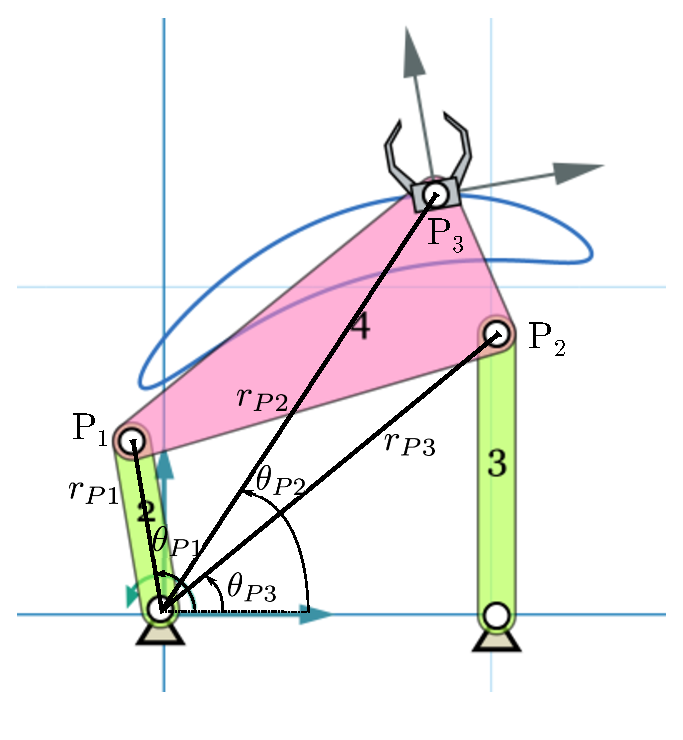
\includegraphics[width=160pt]{jmd-19/figure/fig_fourbar_state.eps}
  \caption{A four-bar linkage with the fixed link of unit magnitude and co-linear with $X$-axis. The polar coordinates of points $P_1, P_2$, and $P_3$ stacked together for $m$ crank orientations constitute the state representation of the four-bar.}
\label{fig_fourbar_state}
\end{figure}


\begin{figure}
\centering
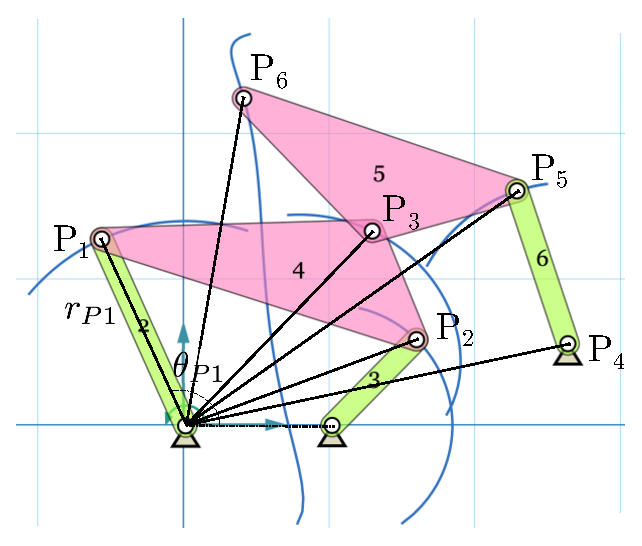
\includegraphics[width=160pt]{jmd-19/figure/fig_sixbar_state.eps}
  \caption{A Stephenson six-bar linkage with the fixed link of unit magnitude and co-linear with $X$-axis. The polar coordinates of points $\{P_i\}_{i=1}^6$ stacked together for $m$ crank orientations constitute the state representation of the six-bar}
\label{fig_sixbar_state}
\end{figure}

In the case of a Stephenson six-bar linkage, we have six points of interest $P_1, P_2, P_3, P_4, P_5, P_6$ as shown in Fig.~\ref{fig_sixbar_state}.
Thus, the state tensor $X$ is given by,
\begin{equation}
  X = \{ r_{P1}, \theta_{P1}, r_{P2}, \theta_{P2}, r_{P3}, \theta_{P3}, r_{P4}, \theta_{P4}, r_{P5}, \theta_{P5}, r_{P6}, \theta_{P6}\}_{i=1}^m,
\end{equation}
where $r_{Pj}$ and $\theta_{Pj}$ are the radial and angular coordinates of point $P_j$. It should be noted that a tuple $(X = \{ r_{P1}, \theta_{P1}, r_{P2}, \theta_{P2}, r_{P3}, \theta_{P3}, r_{P4}, \theta_{P4}, r_{P5}, \theta_{P5}, r_{P6}, \theta_{P6}\}_{i=1}^m,)$ for any of the orientations can be used to construct the original mechanism back.
$X$ has dimensions $[m, 2 \times PoI]$, where $PoI$ is the number of points of interest, whereas, $Y$ is taken as the corresponding coupler path, which has dimension $2m$.


\subsection{Training C-VAE for Mechanism Synthesis}

We flatten $X$ and $Y$ to form vectors of dimensions $m \times 2 PoI$ and $2m$, respectively.
In order to train C-VAE, we pass a batch of $X$ and $Y$ to the network and compute gradients and losses.
The training losses of C-VAE for four-bar and six-bar mechanisms are depicted in Fig.~\ref{fig_cvae_training_loss}.
It can be seen in the Fig.~\ref{fig_cvae_training_loss} that C-VAE for four-bar takes lesser time to train with better training accuracy.
This observation is supported by the fact the six-bar linkages have higher complexities in the distributions of the parameters.

The model architectures and their training results are tabulated in Tables~\ref{tab_cvae_model} and~\ref{tab_cvae_model1} respectively. In Table~\ref{tab_cvae_model} where P. and M. signify path and motion, respectively. This Table also shows the details of each architecture, such as the number of neurons in each layer, the number of hidden layers.

\begin{table*}
  \caption{VAE and C-VAE Models : Architectures (FB=Four-bar, SC=Slider-Crank, SB=Six-Bar)}
\centering
\label{tab_cvae_model}
\begin{tabular}{ccccccc}
\hline
  $(X)$ & X Dim & Name & Enc Arch. & $(z)$ dim  & Dec Arch. & $Y$ \\
\hline
  FB M. & $300$ & C-VAE-M3 & (30) & 3 & (30) & 6 Pts on P. \\
  FB, SC, SB M. & $300$ & C-VAE-M3 & (30) & 3 & (30) & 10 Pts on P.  \\
  FB Linkages & $600$ & C-VAE-LF10 & (300, 100) & 10 & (100, 300) & P. \\
  SB Linkages & $1200$ & C-VAE-LS15 & (600, 300) & 15 & (300, 600) & P. \\
\end{tabular}
\end{table*}

\begin{table*}
  \caption{VAE and C-VAE Models : Training Losses}
\centering
\label{tab_cvae_model1}
\begin{tabular}{ccc}
\hline
  Name & Rec Loss & KL Loss \\
\hline
   C-VAE-M3   & 7.21 & 2.32 \\
   C-VAE-M3   & 10.13 & 3.42 \\
   C-VAE-LF10 & 11.04 & 13.20 \\
   C-VAE-LS15 & 13.02 & 17.34 \\
\end{tabular}
\end{table*}



\begin{figure}
\centering
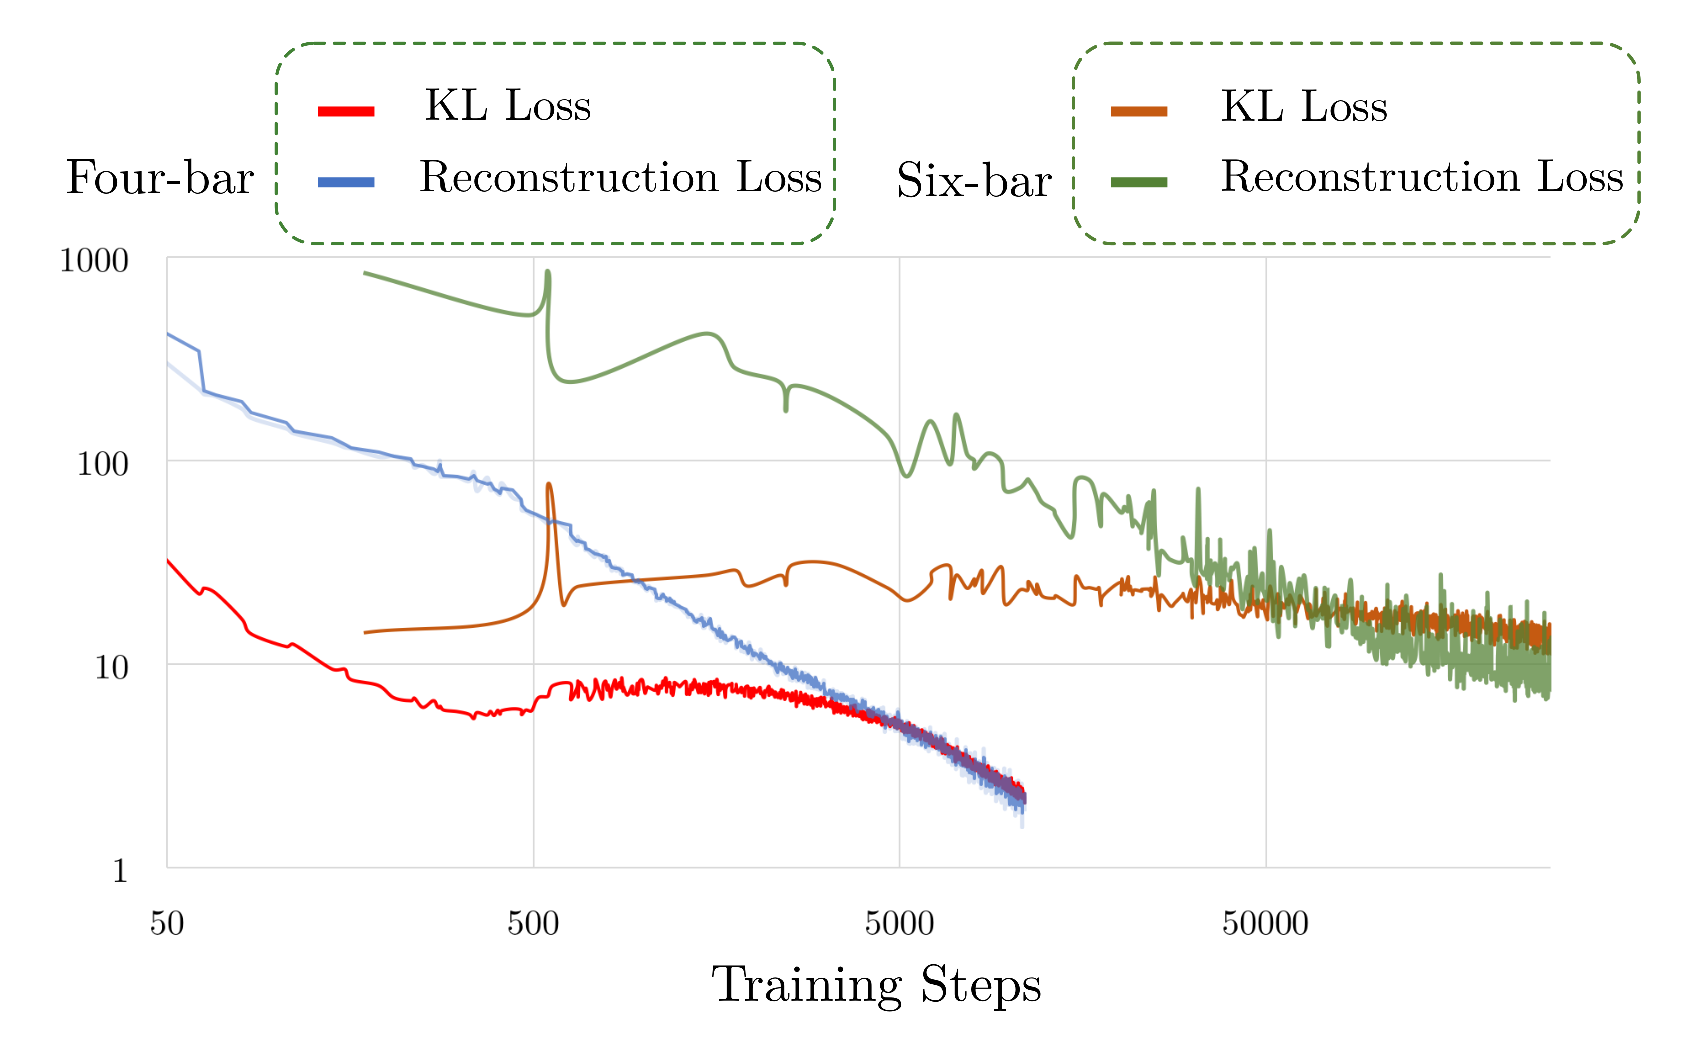
\includegraphics[width=250pt]{jmd-19/figure/fig_cvae_train_loss.eps}
  \caption{Reconstruction and KL Divergence losses for C-VAE-FB and C-VAE-SB. The architectural details of these models are given in Table~\ref{tab_cvae_model}.}
\label{fig_cvae_training_loss}
\end{figure}

\section{End to End Variational Synthesis of Planar Linkages}

\begin{figure}
\centering
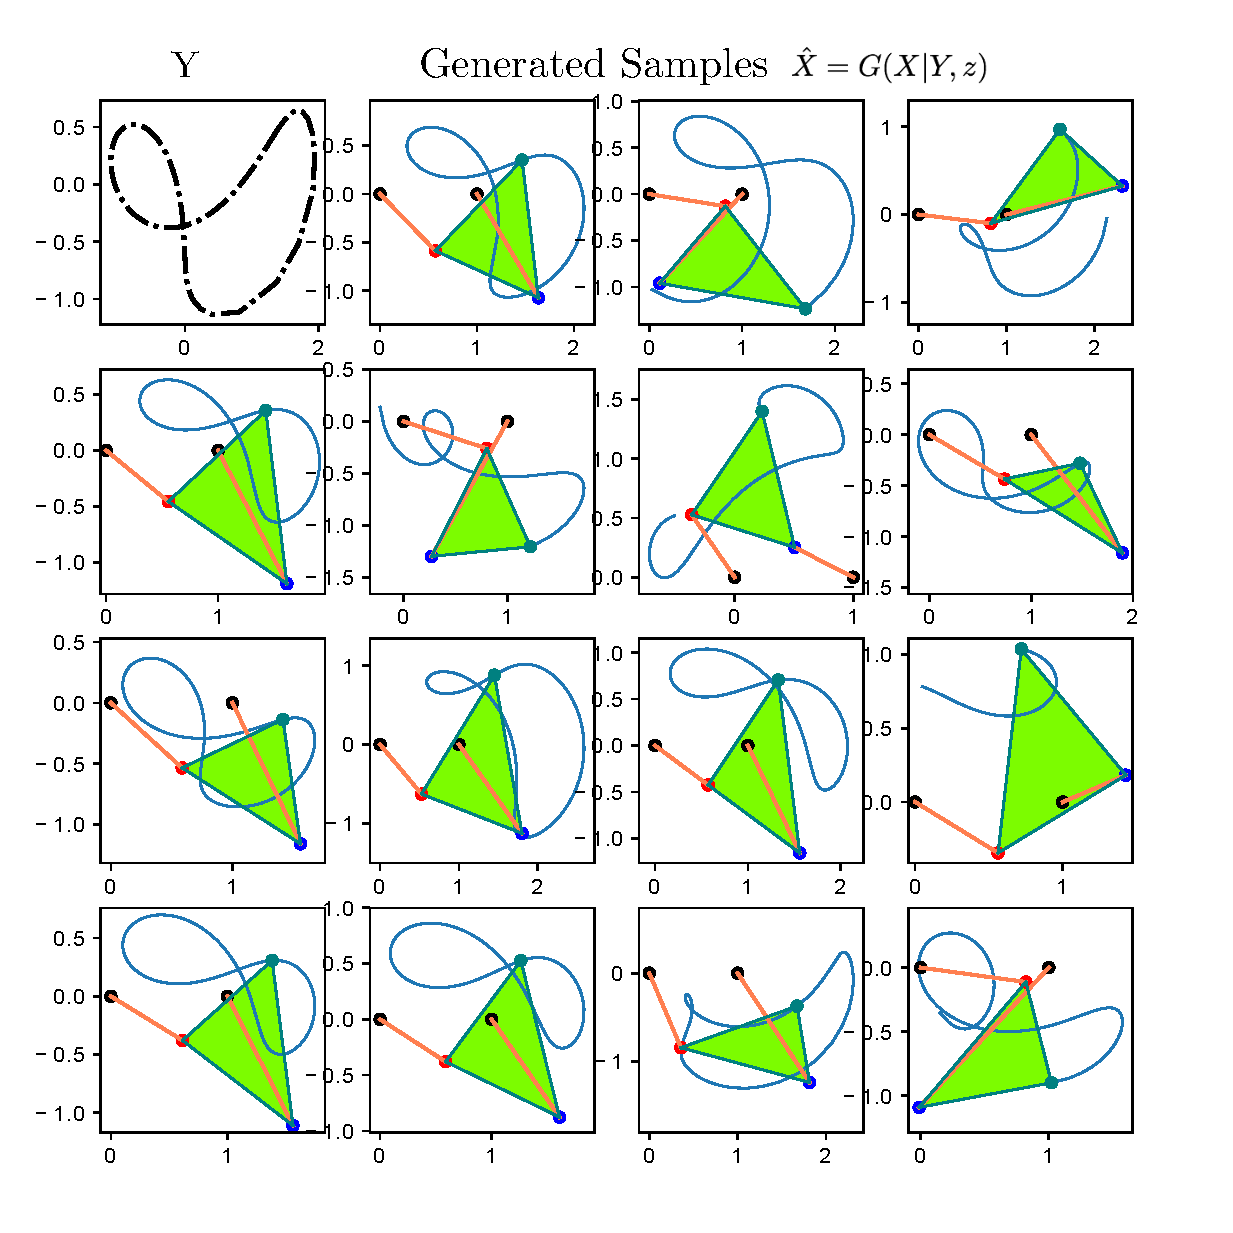
\includegraphics[width=240pt]{jmd-19/figure/fig_end_to_end.eps}
  \caption{Sample linkages generated by C-VAE-LF10 when it is supplied with the conditional coupler curve $Y$ and 10 dimensional Gaussian multivariate $z$. Architecture of this C-VAE is presented in Table~\ref{tab_cvae_model}.}
\label{fig_end_to_end}
\end{figure}
\begin{figure}
\centering
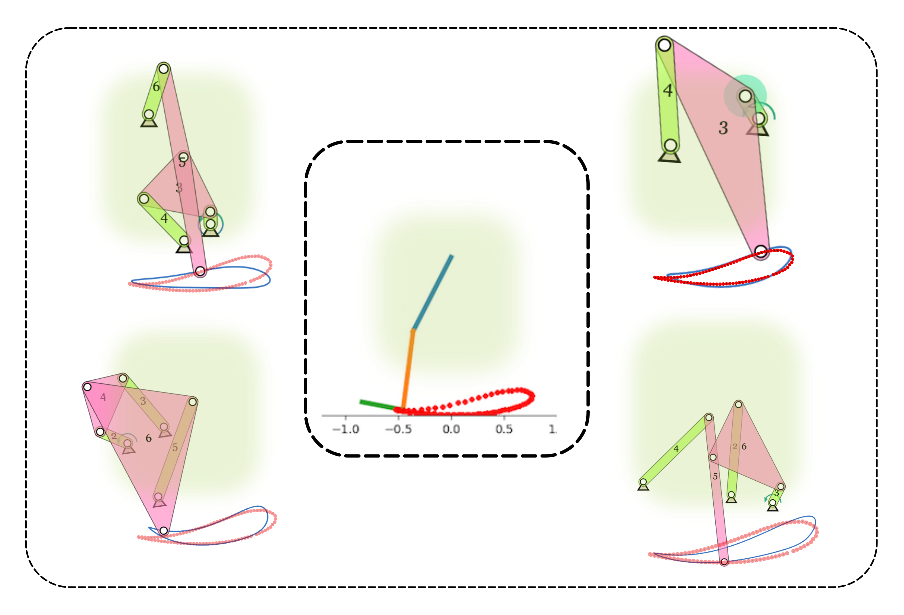
\includegraphics[width=260pt]{jmd-19/figure/fig_sixbar_solutions.eps}
  \caption{Stephenson Six-bars generated by C-VAE-LS15 (see Table~\ref{tab_cvae_model}) conditioned for coupler curve $Y$ and 15 dimensional Gaussian multivariate $z$.}
\label{fig_sixbar_solutions}
\end{figure}
C-VAE is trained to map the probability distribution of linkages to the shape of their corresponding coupler paths.
C-VAE-10 takes a 200-dimensional vector $Y$ and a sample from Gaussian distribution as an input and returns 600-dimensional vector $\hat{X}_{linkage}$ as output. From this 600 dimensional vector, we take the average location of each point of interest and construct the mechanism.
This ensures that each generated sample results in a valid linkage.
There is no guarantee that generated linkage should resemble the path $Y$, but C-VAE is trained to maximize that likelihood.
Figures~\ref{fig_end_to_end} and ~\ref{fig_sixbar_solutions} depict some examples generated by C-VAE when a unseen coupler curve is passed as $Y$ along with a multivariate Gaussian with zero mean and unit variance as $z$ in Eq.~\req{eq_cvae}.
It is interesting to see the variations in the linkage parameters generated by C-VAE.

Combining this model with VAE for coupler trajectory can yield useful planar linkages with variations, making it an End-to-End deep learning model for the variational synthesis of planar linkages.
Further investigation is necessary to make an accurate comparison of this End-to-End deep learning model with classical methods.


\subsection{Case Study}\label{cvae-case-study}
\begin{figure}
\centering
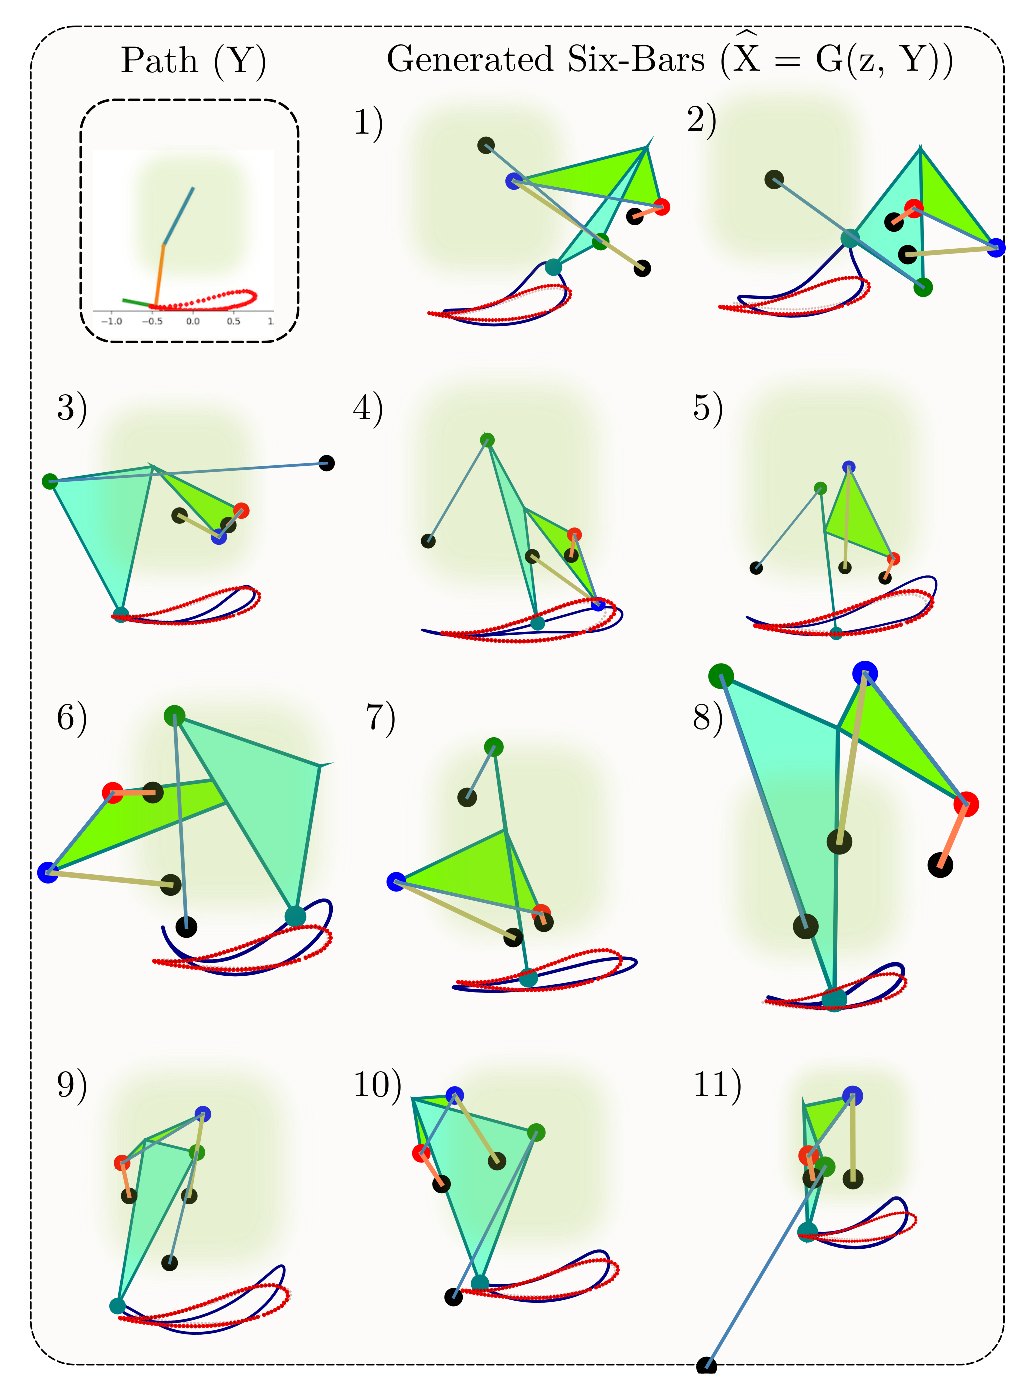
\includegraphics[width=0.7\textwidth]{jmd-19/figure/fig_sixbar_samples.eps}
  \caption{Stephenson Six-bars generated by C-VAE-LS15 (see Table~\ref{tab_cvae_model}) conditioned for coupler curve $Y$ and 15 dimensional Gaussian multivariate $z$. The mechanisms having pivots in desired region are selected for the next step}
\label{fig_sixbar_samples}
\end{figure}

\begin{figure}
\centering
\includegraphics[width=\textwidth]{jmd-19/figure/fig_sixbar_solutions_1.eps}
  \caption{Collection of Feasible Six-Bar Mechanisms with desirable properties. It can be seen that their fixed pivots are in the desired shaded region}
\label{fig_sixbar_solutions_1}
\end{figure}

Now, we use this trained model to generate conceptual designs for the prescribed gait rehabilitation path.
C-VAE generates a conditional distribution of linkages for a given path. A hundred samples from this distribution were taken out of which forty of the samples possessed similar coupler curves as the task curve. From those samples, eleven linkages were selected by visual inspection and displayed in Fig.~\ref{fig_sixbar_samples} along with the prescribed path $Y$.

It should be noted that by avoiding to formulate the problem as minimizing the fitting error between the task path and the coupler curve of the mechanisms, we are able to generate a multitude of mechanisms with desired structure.
Figure~\ref{fig_sixbar_solutions_1} shows a few such feasible mechanisms. It can be seen that some of these mechanisms may have a worse fitting to the task path, but are better suited for this application as their fix pivots lie inside the desired region. Here, the number of  solutions obtained is only limited by the sampling of the latent space; however, not every sample would produce a unique or useful linkage.

\begin{figure}
\centering
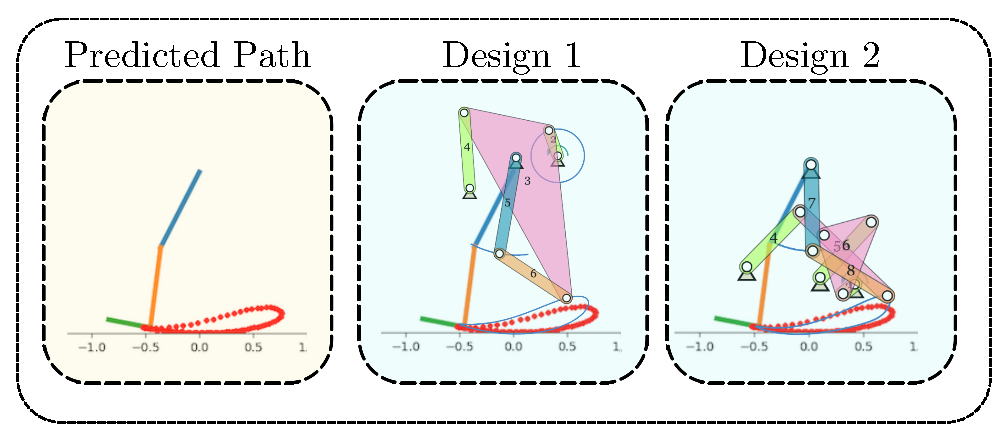
\includegraphics[width=250pt]{jmd-19/figure/fig_final_solutions.eps}
  \caption{Final Linkage Concept Solutions}
\label{fig_final_samples}
\end{figure}

The concepts obtained in Fig.~\ref{fig_sixbar_solutions_1} can be further fine-tuned in detailed design phase.
Along with Six-bars, C-VAE-FB model (see Table~\ref{tab_cvae_model}) was also used to find out the suitable four-bar linkages.
The Fig.~\ref{fig_final_samples} shows one chosen solution concept along with an additional 2R link, which resembles the thigh and lower leg of the person. It can be seen that fixed pivots and link ratios have appropriate proportions with respect to the lower limb of the person. Using the C-VAE approach, we are able to generate a large sample of mechanisms that can satisfy the design requirement. 
